\documentclass[11pt]{report}

%%%%%%%%%%%%%
%% Imports %%
%%%%%%%%%%%%%
\usepackage[a4paper, margin=2cm, top=4cm, bottom=3cm]{geometry}
\usepackage[utf8]{inputenc}
\usepackage[ngerman]{babel}
\usepackage[usenames, dvipsnames]{xcolor}
\usepackage[framemethod=tikz]{mdframed}
\usepackage{listings}
\usepackage{fancyhdr}
\usepackage[acronyms]{glossaries}
\usepackage{tabularx}
\usepackage{booktabs}
\usepackage{cite}
\usepackage{url}

%%%%%%%%%%%%
%% Colors %%
%%%%%%%%%%%%
\definecolor{nordakademie-blue}{RGB}{2,34,94}

%%%%%%%%%%%%%%%%
%% Page Style %%
%%%%%%%%%%%%%%%%
\pagestyle{fancy}
\lhead{\textcolor{nordakademie-blue}{\uppercase{Transferleistung\\ Theorie \& Praxis}}}
\rhead{\textcolor{nordakademie-blue}{
\includegraphics[height=0.85cm,keepaspectratio]{img/NAK-logo}}}
\cfoot{\thepage}
\bibliographystyle{unsrt}
\linespread{1.25}

%%%%%%%%%%%%%%
%% Commands %%
%%%%%%%%%%%%%%
\addto\captionsngerman{\renewcommand{\chaptername}{Abschnitt}}
\newcommand{\inlinecode}{\texttt}
\newcommand*{\SignatureAndDate}[1]{%
    \par\noindent\makebox[2.5in]{\hrulefill}
           \hfill\makebox[2.0in]{\hrulefill}
    \par\noindent\makebox[2.5in][l]{#1}
           \hfill\makebox[2.0in][l]{Datum}
}

%%%%%%%%%%%%%%%%%%%%%%
%% Glossary entries %%
%%%%%%%%%%%%%%%%%%%%%%
\newacronym{bundler}{WAB}{Web Application Bundler}
\newacronym{app}{Web App}{Web Application}
\newacronym{js}{JS}{JavaScript}
\newacronym{html}{HTML}{HyperText Markup Language}
\newacronym{css}{CSS}{Cascading Style Sheets}
\newacronym{cdn}{CDN}{Content delivery network}
\newacronym{hmr}{HMR}{Hot Module Replacement}
\newglossaryentry{cpuTime}
{
  name=CPU-Zeit,
  description={ist die Zeit in welcher ein Prozess die CPU beansprucht hat. Sie unterscheidet sich von der normalen Zeit dahingehend, dass Nutzungen des Prozessors durch andere Prozesse nicht mit einfließen.},
  plural=CPU-Zeiten
}
\makeglossaries
\makeindex

%%%%%%%%%%%%%%
%% Document %%
%%%%%%%%%%%%%%
\begin{document}

    %%%%%%%%%%%%%%%
    %% Frontpage %%
    %%%%%%%%%%%%%%%
    {\huge Transferleistung 1}
    \vspace{1cm}

    \begin{center}
        \begin{tabularx}{\textwidth}{r|X}
            Matrikelnummer & 8252 \\\midrule
            Thema & Optimierung der Build-Dauer eines Web Application Bundler durch Anpassung der Konfiguration und dessen Auswirkung auf den Entwicklungsprozess \\\midrule % TODO Add topic to front page
            Studiengang, Zenturie & Angewandte Informatik, A17b\
        \end{tabularx}
    \end{center}
    \pagebreak

    \tableofcontents
    \listoffigures
    \listoftables
    \pagebreak

   	%%%%%%%%%%%%%
    %% Content %%
    %%%%%%%%%%%%%
    \chapter{Einleitung}
    	In der Software-Entwicklung werden häufig Module von anderen Entwicklern in einem Projekt verwendet. Da es in der Web-Entwicklung im Bereich von \Gls{js}, \Gls{html} und \Gls{css} keinen Build-Prozess gibt werden in der klassischen Web-Entwicklung Abhängigkeiten entweder direkt von sogenannten \Glspl{cdn} eingebunden oder manuell heruntergeladen und in das Projekt kopiert.\\
		Alternativ können Abhängigkeiten per Package-Manager (z.B. \emph{npm} oder \emph{yarn}) heruntergeladen werden und in einem Bundling-Prozess mit den vorhandenen Modulen des Projektes zu einer Datei kombiniert werden. Dazu werden \Glspl{bundler} wie zum Beispiel \emph{Webpack} oder \emph{ParcelJS} verwendet.\\
		Zusätzlich zu der Konkatenation von Modulen übernehmen solche Tools die Transformation und Transpilation von Eingabedateien um z.B. Textdateien oder Bilder in den Code zu integrieren, Dateien zu optimieren und komprimieren oder Module, welche in neuen \Gls{js} oder \Gls{css} Versionen geschrieben wurden, in alte Versionen zu übersetzen um Kompatibilität mit älteren Browsern zu gewährleisten.\\
			% Good place to use sources why this is done
		\\
    	Dieses Transferleistung befasst sich mit der Beeinflussbarkeit der Build-Zeit eines \Gls{bundler} durch Anpassungen an der Konfiguration in Bezug auf die Geschwindigkeit des Softwareenwicklungsprozess. Ein \Gls{bundler} ist ein Tool, welches sämtliche Ressourcen und Abhängigkeiten einer \Gls{app} analysiert und in wenige Ausgabedateien zusammenfasst. Dabei werden optional Optimierungsschritte durchgeführt um die Anzahl und Größe der Ausgabedateien zu reduzieren. Sowohl die Analyse der Abhängigkeiten als auch das Bundling und die Optimierung können durch Konfigurationsdateien angepasst werden. In dieser Arbeit werden die folgenden Forschungsfragen näher beleuchtet:
	    	\begin{enumerate}
		    	\item Ist die Build Performance relevant für den Entwicklungsprozess?
		    	\item Welche Faktoren haben eine Auswirkung auf die Dauer des Build? \label{question1}
		    	\item Lassen sich diese Faktoren in einem Software-Projekt beeinflussen?
		    \end{enumerate}

		\section{Relevanz für die PPI AG}
			Bei der PPI AG gibt es mehrere Projekte, welche unter anderem die Entwicklung einer Web-App umfassen. Dies schließt zum Beispiel das Studenten-Verwaltungstool StuMaTo ein, welches der Verwaltung und Verteilung von Aufgaben an die Studenten dient. Dieses Tool wird in der kommenden Praxisphase von einem kleinen Team aus Studenten weiterentwickelt werden, wobei eine direkte Relevanz der Ergebnisse dieser Transferleistung sich positiv auf den Entwicklungsprozess auswirken könnte.
			% TODO Problemstellung verteidigen: Projekttools meist vorgegeben daher Optimierung des Prozess
	
		% \section{Relevanz der Build Dauer}
		% 	To be done. % TODO Write this argument

		\section{Methodik}
			Um die Forschungsfrage \ref{question1} zu beantworten ist ein Projekt nötig an dem die Forschung durchgeführt werden kann.
			\subsection{Beispiel-Projekt}
				Im Rahmen dieser Transferleistung wird eine rudimentäre \Gls{app} aufgesetzt, welche sich vom Umfang auf die für den Build Prozess relevanten Kriterien beschränkt und eine Analyse der Faktoren ermöglichen soll, welche einen Einfluss auf die Build Zeit haben.

				\paragraph{Bundling Tool} In vielen Projekten wird die zu nutzende Technologie meist von Projektleitern oder Kunden vorgeschrieben. Entsprechend wurde für dieses Projekt der am weitesten verbreitete\footnote{\url{http://www.npmtrends.com/webpack-vs-parcel-bundler-vs-rollup-vs-browserify}} \Gls{bundler} \emph{Webpack} verwendet um eine möglichst einfache Übertragung der Konfigurationsoptionen auf andere Projekte zu ermöglichen.

				\paragraph{React} Bei der Entwicklung von \Glspl{app} werden häufig Frameworks wie z.B. jQuery, React, Angular oder VueJS verwendet. In diesem Projekt wird \emph{React} aufgrund seiner Popularität\footnote{\url{http://www.npmtrends.com/angular-vs-ember-source-vs-react-vs-vue}} und den vorhandenen Kenntnissen des Authors verwendet.

				\paragraph{Material UI} Als Library für grafische Komponenten wurde das Projekt \emph{Material UI}\footnote{\url{https://material-ui.com}} gewählt, da es aufgrund der vorhandenen Beispiel in der Dokumentation ein schnelles Prototyping der Dummy-UI ermöglicht. Außerdem wurde die Schriftart Roboto und das Material-UI Icon-Set von Google eingebunden, da sie den UI Guidelines\footnote{\url{https://material.io/design/introduction}} der Library entsprechen und von dieser empfohlen werden.

				\paragraph{Victory Graphs} Um den Umfang des Projektes zu erweitern und ein möglichst realistisches Szenario für die Build-Zeit zu erreichen wurde zusätzlich eine Abhängigkeit für Diagramme eingebunden. Hierbei wurde \emph{Victory}\footnote{\url{https://formidable.com/open-source/victory/}} gewählt, da es eine einfache und gut dokumentierte Integration mit React bietet.

			\subsection{Messverfahren}
				Die Dauer des Build wird der Ausgabe des Build-Tool Webpack entnommen. Um eventuelle Ungenauigkeiten durch Unterschiede in der Prozessorauslastung oder eventuelle Caches zu minimieren wird der Build mehrfach ausgeführt und die durchschnittliche Dauer berechnet. Dabei wird der erste Build nach Anpassung der Konfigurationsdatei nicht mit in die Wertung einbezogen, da er mögliche Abweichungen durch Caching der neuen Einstellungen aufweisen könnte. Anschließend werden für jeden Datenpunkt jeweils zwei Builds ausgeführt um ein realistisches Szenario zu schaffen. Der erste Build wird dabei mit der Ausgangslage des Projekt durchgeführt. Im Anschluss wird der Inhalt einer Datei verändert und ein weiterer Vorgang gestartet. Die \Gls{cpuTime}, die dieser zweite Build benötigt, wird gemessen und in die Wertung aufgenommen.
				% TODO Name a fixed number of runs (10)
				% TODO Note the capturing of a memory usage profile
				% TODO Reference the script on GitHub
	
				\paragraph{Gerät} Sämtliche Builds werden auf einem Retina MacBook aus dem Jahr 2017 mit 8GB RAM und einem Intel Core i7 mit macOS 10.14 durchgeführt. Während des Build werden sämtliche Anwendungen, welche nicht für die Ausführung des Betriebssystems oder des Builds kritisch sind, geschlossen um eine möglichst reproduzierbare Umgebung zu schaffen. Es wird dabei darauf geachtet, dass das Gerät während der Messungen an eine Stromquelle angeschlossen und ausreichend gekühlt ist, um CPU throttling zu vermeiden.

			\subsection{Gruppierung der Anpassungen}
				Die Analyse der möglichen Optimierungen wird in mehreren Schritten durchgeführt.
				\paragraph{Grundlage}\label{baseline-build} Zu Beginn wird das Beispiel Projekt mit einer Konfiguration gebaut, welche einer typischen Produktionsumgebung ähnelt. Die resultierende Build Dauer wird als Grundlage für den Vergleich mit potentiellen Optimierungen genommen, welchen in den folgenden Schritten durchgeführt werden.

				\paragraph{Umgebungsunabhängig} Als zweiter Schritt werden verschiedene Aspekte der Konfigurationsdatei angepasst, welche keine signifikanten Auswirkungen auf die resultierenden Build-Artefakte haben\footnote{Die Größe der Ausgabedatei darf um nicht mehr als $5\%$ abweichen und die Browser-Kompatibilität sowie Funktionalität nicht beeinträchtigt werden.}, und ihre individuellen Auswirkungen unabhängig voneinander gemessen.

				\paragraph{Destruktive Anpassungen} Einige Änderungen haben negative Auswirkungen auf die resultierenden Build-Artefakte, wie zum Beispiel eine größere Ausgabedatei oder verminderte Browser-Kompatibilität, aber die Funktionalität in einer Entwicklungsumgebung nicht beeinträchtigen. Im dritten Schritt werden Anpassungen vorgenommen, welche solch negativen Auswirkungen haben. Diese werden wie zuvor unabhängig voneinander gemessen.

				\paragraph{Gesamtbewertung} Im letzten Schritt werden sämtliche Änderungen die eine Verbesserung der Build-Zeit von $>=5\%$ bewirkt haben gemeinsam angewendet. Dies wird zuerst für die umgebungsunabhängigen Anpassungen und anschließend für alle durchgeführt. Dies dient dazu eventuelle Interaktionen von Konfigurationsänderungen abzudecken und einen Gesamtwert für die Verbesserung in der Build-Zeit zu erhalten.

	\clearpage

	\chapter{Durchführung}
		\section{Ausgangslage}
			Wie auf Seite \pageref{baseline-build} erwähnt wurde zunächst eine Basismessung durchgeführt. Die genutzte Konfigurationsdatei kann auf GitHub\footnote{https://github.com/TexNAK/WebBundlerOptimization/blob/d018b3e0db6a861c4f41e38e7265ca8f9d500319/webpack-project/webpack.config.js} gefunden werden.
			\paragraph{Abbildung \ref{figure:baseline_duration}} zeigt die \Gls{cpuTime} der einzelnen Ausführungen. Auf der X-Achse sind die einzelnen Läufe verteilt. Die Y-Achse stellt die gemessene Zeit dar, welche in Systemzeit (also Zugriffe auf die Kernel API) und Nutzerzeit geteilt. Die Abbildung zeigt eine durchschnittliche Zeit von 26 Sekunden mit einer maximalen Abweichung von $3\%$. Aufgrund der geringen Abweichung in Verteilung und Gesamtdauer wird in den nachfolgenden Messungen nur die durchschnittliche Dauer betrachtet.
			\paragraph{Abbildung \ref{figure:baseline_memory}} zeigt den Speicherverbrauch des \Gls{bundler}, wobei die X-Achse die vergangene Zeit seit Prozessstart und die Y-Achse den Speicherverbrauch in Megabyte darstellt. Auch bei diesem Graph ist nur eine geringe Abweichung vom Durchschnitt zwischen den einzelnen Durchgängen sichtbar.
			% TODO Cite smth that defines what User and System time are
			\begin{figure}
                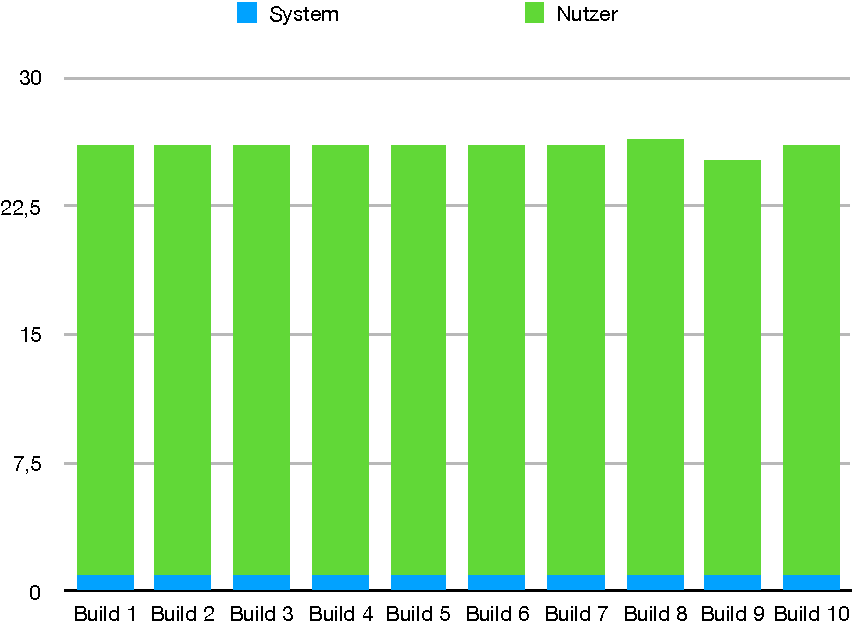
\includegraphics[width=\textwidth]{img/baseline_duration.pdf}
                \caption{Basismessung | CPU Zeit}
                \label{figure:baseline_duration}
            \end{figure}
            \begin{figure}
                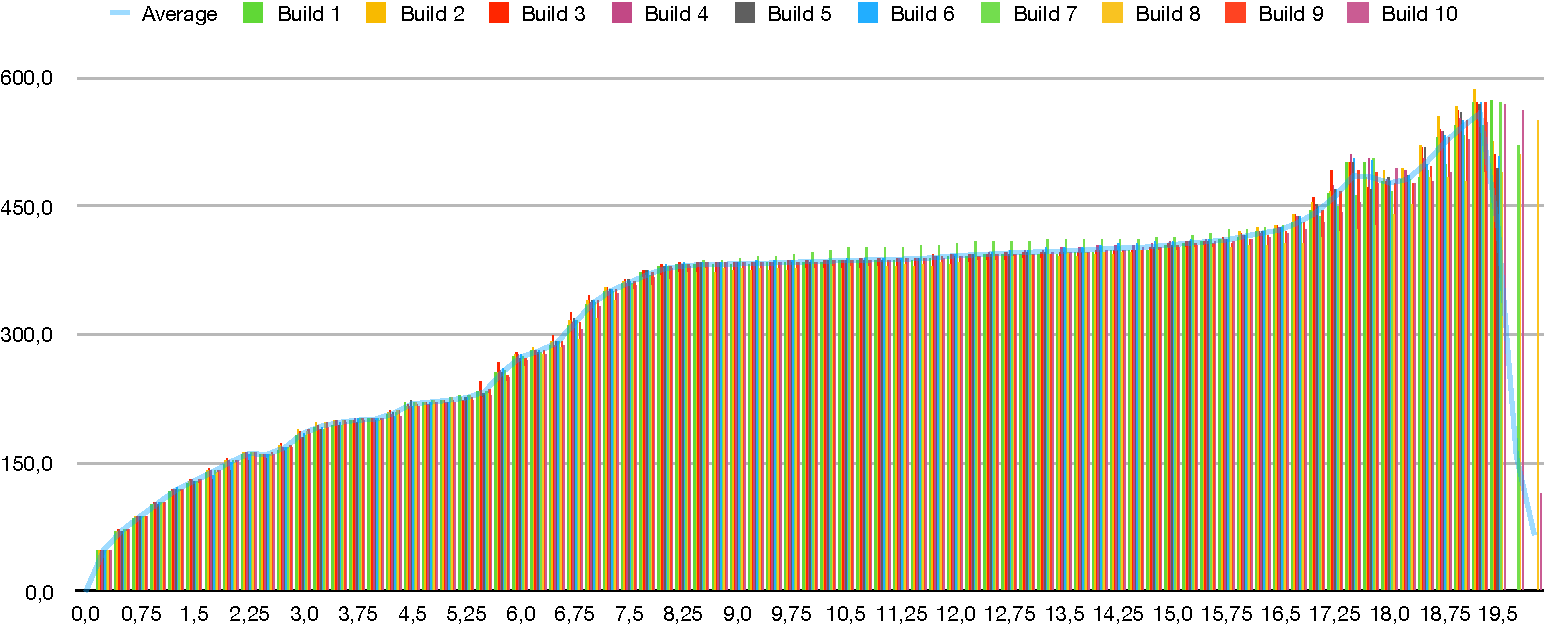
\includegraphics[width=\textwidth]{img/baseline_memory.pdf}
                \caption{Basismessung | Speicherverbrauch}
                \label{figure:baseline_memory}
            \end{figure}

        \section{Nicht destruktive Anpassungen}
        	\subsection{Optimierung der Minification}
        	\subsection{Scoped compilation}
        		% DLL Plugin
    		\subsection{Caching}
    			% cache-loader

    	\section{Destruktive Anpassungen}
    		\subsection{Source-Maps}
    		\subsection{Inkrementelle Builds}
    		\subsection{In-Memory-Compilation}
    		\subsection{\Gls{hmr}}

		\section{Gesamtbewertung}
			\subsection{Umgebungsunabhängig}
			\subsection{Destruktiv}

	\chapter{Auswertung}
		Let's hope it got improved! % TODO Evaluate what happened
		
		\section{Beeinflussbarkeit der Build Dauer}
			To be done. % TODO Write this argument
			% Note the following which broadens the applicability of the results:
			%  Da Webpack wie die meisten \Glspl{bundler} intern Tools wie z.B. BabelJS\footnote{https://babeljs.io} oder UglifyJS\footnote{http://lisperator.net/uglifyjs/} ausführt sollte es möglich sein ein Großteil der aufgedeckten

		\section{Zusammenfassung}
			Whatever. % TODO What have we learned?
    \pagebreak

    %%%%%%%%%%%%%%
    %% Appendix %%
    %%%%%%%%%%%%%%
    \hspace{0pt}
    \vfill
    \subsection*{Eidesstattliche Erklärung}
        Hiermit erkläre ich an Eides statt, dass ich die vorliegende Arbeit ohne Hilfe Dritter und ohne Benutzung anderer als der angegebenen Hilfsmittel angefertigt habe. Die aus fremden Quellen direkt oder indirekt übernommenen Gedanken sind als solche kenntlich gemacht. Die Arbeit wurde bisher in gleicher oder ähnlicher Form weder von mir noch von jemand anderem als Prüfungsleistung vorgelegt.
        \vspace{2cm}
        \SignatureAndDate{Unterschrift}
    \vfill
    \hspace{0pt}
    \pagebreak

    \glsaddall
    \printglossary
    \printglossary[type=\acronymtype]
    \pagebreak

    \nocite{*}
    \bibliography{main.bib}

\end{document}
